\section{Распределённая файловая система. HDFS. Архитектура. Особенности, сценарии спользования. Достоинства и недостатки.}

\D{
    DFS - распределенная файловая система.
	
	Цели:
	\begin{itemize}
		\item Распространить файлы по нескольким машинам.
		\item Добавить отказоустойчивость при падении одной машины.
		\item Балансировать нагрузку.
	\end{itemize}
}

\begin{figure}[h]
	\centering
	\begin{minipage}[b]{0.8\textwidth}
		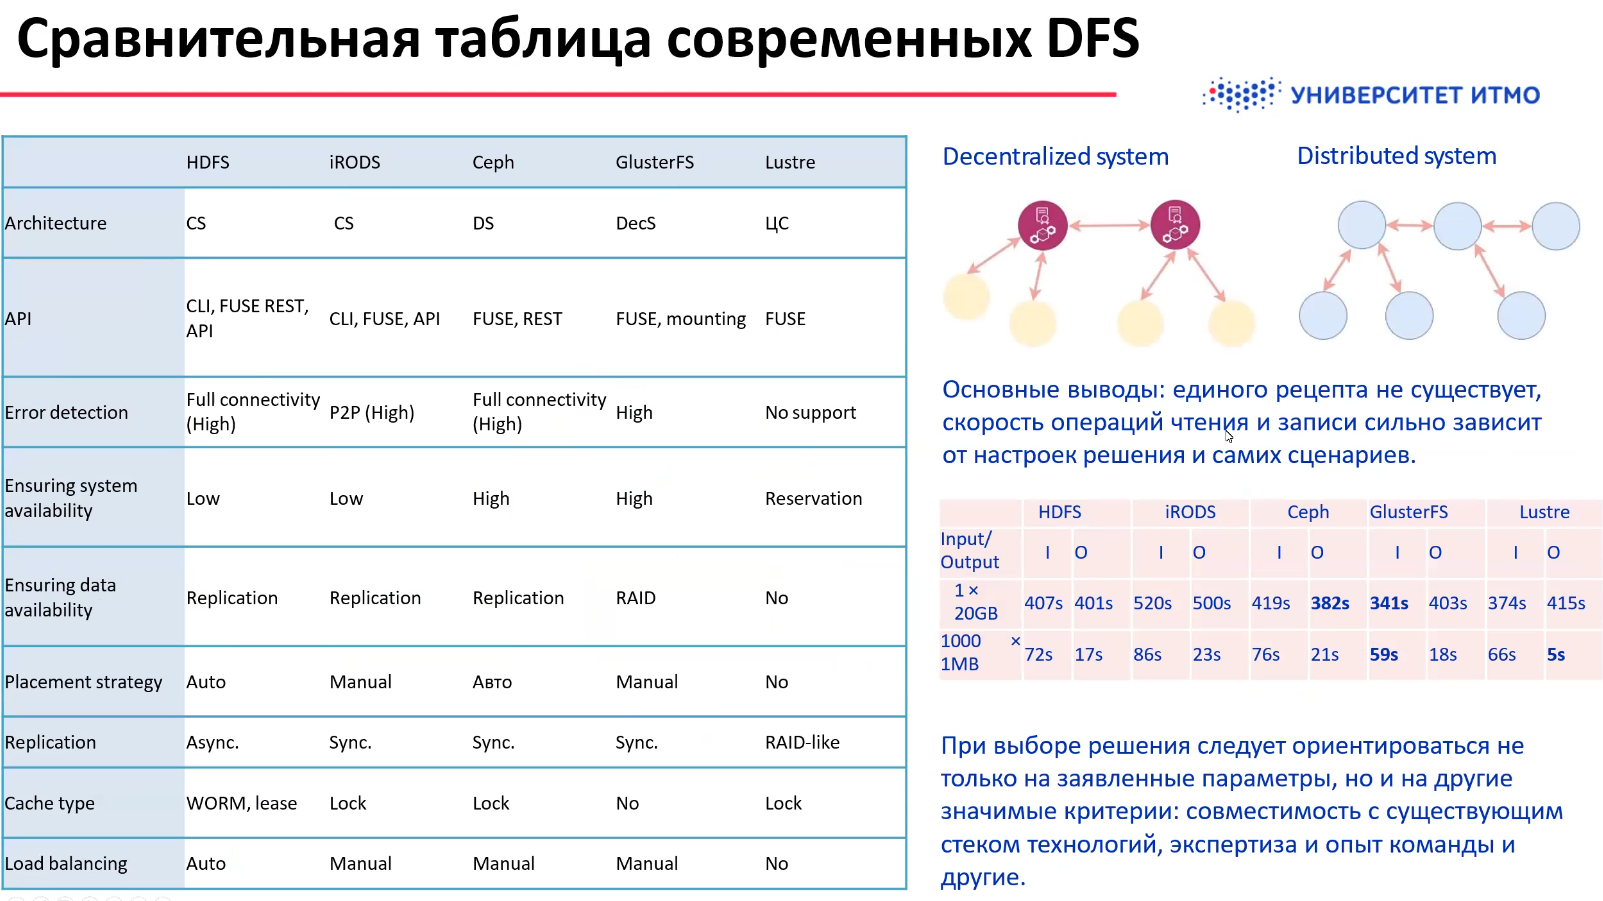
\includegraphics[width=\textwidth]{images/dfs.png}
		\caption{Сравнение DFS}
	\end{minipage}
\end{figure}

\subsection*{Облачне хранилища}

Подразумевается система с поддержкой протокола S3 (хранит объекты).

\begin{figure}[h]
	\centering
	\begin{minipage}[b]{0.8\textwidth}
		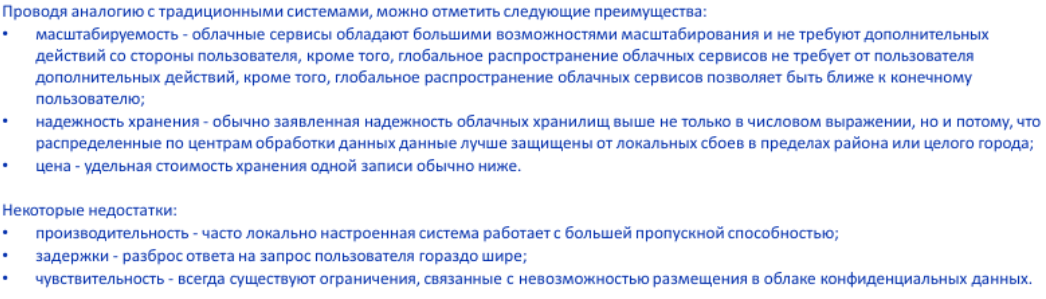
\includegraphics[width=\textwidth]{images/s3dfs.png}
		\caption{S3 vs DFS}
	\end{minipage}
\end{figure}

\subsection*{HDFS}

\D{
	HDFS (hadoop DFS) - иерархия каталогов для хранения
	больших объемом с возможностью потокового доступа,
	поблочно распределенной по узлам.
}

MapReduce + DFS.

\subsection*{HDFS Архитектура}

Реализует архитектуру Master-Slave.

\textbf{Управляющий узел (сервер имен)} - единственный в
кластере узел с ПО для управления пространством имен ФС,
хранящий дерево файлов.

\textbf{Secondary NameNode} - копирует мастер для восстановления.

\textbf{DataNode} - отвечает за запись и чтение данных,
выполнение команд от NameNode, отправку сообщений о состоянии,
обработку запросов read/write.

\textbf{Client} - взаимодействует через API с ФС.

Особенности:
\begin{itemize}
	\item большой размер блока
	\item отказоустойчивость
	\item репликация на уровне кластера
	\item асинхронная репликация
	\item потоковое считывание
	\item однократная запись
	\item самодиагностика
\end{itemize}

недостатки:
\begin{itemize}
	\item сервер имен является центральной точкой всего кластера и его
	отказ повлечет сбой системы целиком;
	\item отсутствие полноценной репликации Secondary NameNode;
	\item отсутствие возможности дописывать или оставить открытым
	для записи файлы в HDFS, за счет чего в классическом
	дистрибутиве Apache Hadoop невозможно обновлять блоки уже
	записанных данных;
	\item отсутствие поддержки реляционных моделей данных;
\end{itemize}